\section{Background and Related Work}\label{sec:background}

%% In this section, we introduce the concepts and terminology that are necessary to understand the reminder of this paper. First, Section~\ref{sec:sand} introduces some background information about \emph{sandboxes} within the security context. Section~\ref{sec:repackage} presents background information about repackaged application and how they introduce malicious behavior.
%% Finally, in Section~\ref{sec:android-sandbox} we review the \emph{mining sandbox approach} for detecting repackaged Android apps.

There are many tools that favor developers to reverse engineering the Android bytecode language~\cite{DBLP:conf/issta/WangGMC15}.
For this reason, software developers can easily decompile trustworthy apps, modify their contents by inserting malicious code,
repackage them with malicious payloads, and re-publish them in app stores, including official ones like the Google Play Store.
It is well-known that repackaged Android apps can leverage the popularity of real apps to increase their propagation and spread malware~\cite{DBLP:journals/tse/LiBK21}. As an example, in 2016 a repackaged version of the famous Pokémon Go app was discovered less than 72 hours after the game was officially released in the United States, Australia, and New Zealand~\cite{DBLP:journals/tse/LiBK21}. The repackaged version, originated from an unofficial app store, gained full control over the victim's phone, obtaining access to main functions such as the phonebook, audio recorder, and camera.

Repackaging has been raised as a noteworthy security concern in Android ecosystem by stakeholders in the app development industry and researchers~\cite{DBLP:journals/ese/KhanmohammadiEH19}. Indeed, there are reports claiming that about 25\% of Google Play Store app content correspond to repackaged apps~\cite{DBLP:conf/sigmetrics/ViennotGN14}. Nevertheless, all the workload to detect and remove malware from markets by the stores (official and non-official ones), have not been accurate enough to address the problem. As a result, repackaged Android apps threaten security and privacy of unsuspicious Android app users, beyond compromising the copyright of the original developers~\cite{DBLP:journals/access/KimLCP19}. Aiming at
mitigating the threat of malicious code injection in repackaged apps,
several techniques based on both static and dynamic analysis of Android apps have been proposed,
including the \mas for malware classification~\cite{DBLP:conf/icse/JamrozikSZ16,DBLP:conf/wcre/BaoLL18}. 





\subsection{Mining Android Sandboxes}\label{sec:android-sandbox}

A \emph{sandbox}
is a well-known mechanism to secure a system and forbid a software component from accessing
resources without appropriate permissions. Sandboxes have also been used to build an isolated
environment within which applications cannot affect other programs, the network, or other device
data~\cite{DBLP:journals/peerj-cs/MaassSCS16}. The idea of using sandboxes emerged from the
need to test unsafe software, possible malware, without worrying about the integrity of the
device under test~\cite{DBLP:conf/esorics/BordoniCS17}, shielding the operating system from security issues.
To this end, a sandbox environment should have the minimum requirements to run the
program, and make sure it will never assign the program more privileges than it should have,
respecting the \emph{least privilege} principle.
% This principle ensures unauthorized access to resources,
% improving the system's overall health.
Within the Android ecosystem, sandbox approaches ensure the principle
of the \emph{least privilege} by preventing apps from having direct access to resources like device hardware (e.g., GPS, Camera), or sensitive data from other apps. Access to sensitives data
like contact list or resources are granted through specific APIs, known as sensitive APIs, which are managed by by coarse-grained Android permissions system~\cite{DBLP:journals/corr/abs-2109-06613}.



%% The main market source for Android apps is Google Play Store. Unfortunately, it has
%% a flexible policy regarding the process of publishing apps, and therefore, many Android apps are removed from the
%% store because of issues related to malware\cite{DBLP:conf/msr/WangLL0X18}. Google Play tries
%% to minimize unauthorized access to sensitive resources by malicious apps,
%% listing each app with its requested permission. {\color{red}Those permissions are presented to Android
%% users at app installation moment since version 6}. However, some works presented that most users are careless regarding these permissions since they are only interested to run the app~\cite{DBLP:conf/soups/FeltHEHCW12}. This represents a great security breach since malware usually asks for more permissions than their APIs normally would require~\cite{DBLP:conf/ccs/FeltCHSW11}.

%% \begin{figure}[ht]
%% \centering
%% 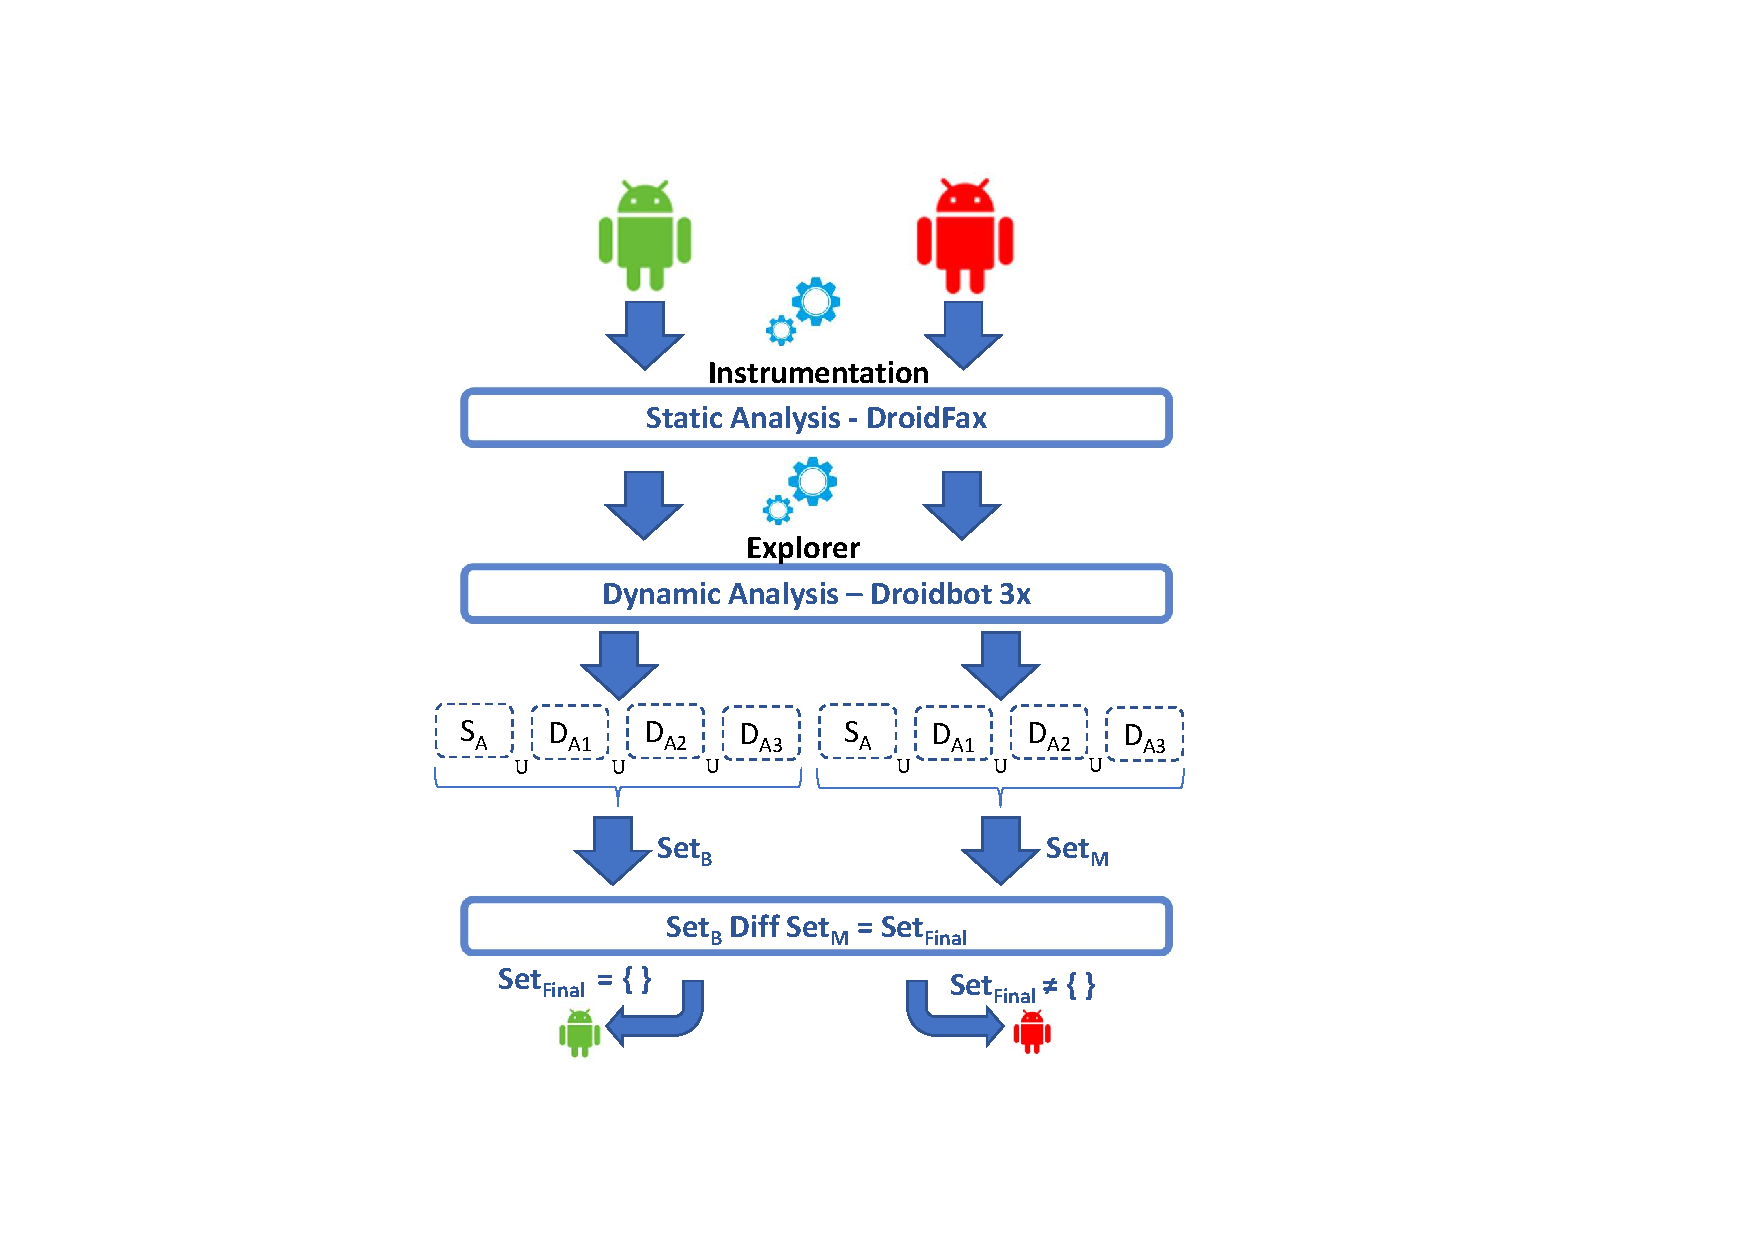
\includegraphics[scale=0.35]{images/mineSandbox.pdf}
%% \caption{Mine Sandbox.}
%%  \label{fig:mineSandbox}
%% \end{figure}

The \mas~\cite{DBLP:conf/icse/JamrozikSZ16} aims at automatically
building a sandbox through dynamic analysis (i.e., using automatic test generation tools).
The main idea is to grant permissions to an app based on its calls to sensitive APIs.
Thus, sandboxes build upon these calls to create safety rules and then block future
calls to other sensitive resources, which diverge from those found in the first exploratory
phase. Using the Droidmate test generation tool~\cite{DBLP:conf/icse/JamrozikZ16},
Jamrozik et al. proposed a full-fledged
implementation of the \mas, named Boxmate~\cite{DBLP:conf/icse/JamrozikSZ16}. 
Boxmate records the occurrences of calls to sensitive APIs and, optionally, the UI
events (e.g., a button click) that trigger these calls. Therefore, it is possible to configure Boxmate to record events associated with each sensitive call as
tuples (event, API), instead of recording just the set of calls to sensitive APIs. Jamrozik et al. argue that, in this way, Boxmate generates finer
grain results, which
might improve the accuracy of the \mas---even with the presence of reflection, a feature commonly used in
malicious apps~\cite{DBLP:conf/issta/0029BOK16}.

In fact, the \mas can be implemented using
a mix of static and dynamic analysis. In the first phase, one
can instrument an Android app to log any call to the Android sensitive methods.
After that, one can execute a test case generation tool (such as DroidMate, DroidBot, or Monkey) to explore the app behavior at runtime,
while the calls to sensitive APIs are recorded.
%Figure~\ref{fig:mineSandbox} presents this general approach for \mas.
This set of calls to sensitive APIs is then used
to configure the sandbox. The general \mas % (see Figure~\ref{fig:mineSandbox})
suggests that the more efficient the test generation tool (for instance, in terms of code coverage),
the more accurate would be the resulting sandbox.


%\todo[inline]{Since this figure is not discussed in the paper, we can remove it without any problem. I have enriched the previous paragraph, though, to make it
%  more necessary. Nonetheless, I will change this figure a bit, in order to
%represent the instrumentation phase.}

\subsection{Mining Android Sandbox for Malware Classification}

Besides being used to generate Android sandboxes, the \mas is also effective 
to detect if a repackaged version of an Android app contains malicious
behavior~\cite{DBLP:conf/wcre/BaoLL18}. In this scenario, the \emph{effectiveness} of the approach
is estimated in terms of the accuracy in which malicious behavior is correctly identified in the repackaged version of the
apps.


%Figure~\ref{fig:sensitiveAPI} illustrates the \mas for
%repackaged apps identification.
%We leverage DroidXP~\cite{DBLP:conf/scam/CostaMCMVBC20} to collect the set of sensitive APIs
%the versions of the apps call (benign/malign versions).
The \mas for malware classification typically works as follows. In a first step ({\bf instrumentation phase}), 
a tool instruments the code of the apps (both original and repackaged versions) to collect relevant information
during the apps execution in later stages. Then, in a second step ({\bf exploration phase}),
the \mas collects a set $S_1$ with all calls to sensitive APIs the original version of an app executes while running a test case generator tool (like DroidBot).
In the third step ({\bf exploitation phase}), the \mas (a) collects a set $S_2$ with all calls to sensitive APIs the repackaged version of an app
executes while running a test case generator tool and then (b) computes the set $S = S_2 \setminus S_1$ and checks whether  $S$ is empty or not.
The \mas classifies the repackaged version as a malware whenever $|S| > 0$.  

%%We configure DroidXP to run DroidBot for $3$ minutes. Since some malware may use dynamic features (such as reflection) to introduce malicious behavior,
%%which can change apps behavior at runtime~\cite{DBLP:journals/spe/ZhangLTX18,DBLP:journals/tosem/LiTX19}, this second
%%analysis is also important to disclose some sensitive APIs calls ignored by first analysis (static analysis).

%%While our static analysis is made once, we execute dynamic analysis $3$ times. The result of static analysis and all executions is finally joined, forming a final set containing all calls to sensitive APIs coming from the original version of the app, as described at Figure~\ref{fig:sensitiveAPI}: ($S_{A}$, $D_{A1}$, $D_{A2}$, $D_{A3}$). We carry out the same procedure for the malicious version of the apps, creating a distinct set of calls to sensitive APIs (now coming from the malicious version of the apps). In a final step, we compare the two sets of calls to sensitive APIs ($Set_B, Set_M$). We use the following rules to check for a malicious behavior. 

%% \begin{enumerate}
%%     \item If the difference between the two final sets is an empty set, we cannot distinguish the benign from the malicious version of the app (false negative).
%%     \item Otherwise, we successfully distinguish the benign from the malicious version of the app (true positive). 
%%     %\kn{Cant we replace the first part of the second point simply as "Otherwise" or is there some specific corner cases that I am missing}
%% \end{enumerate}

%% In addition, this procedure also enables us to identify the calls to sensitive APIs that are more frequently injected by the malicious version of the apps
%% in our dataset. 

%% %\fh{here I have to insert the figure}

%%\begin{figure}[ht]
%%\centering
%%\includegraphics[scale=0.45]{images/sensitiveAPIdiff.pdf}
%%\caption{All procedure for suspicious app identification %%using sensitive API set diff.}
%%\label{fig:sensitiveAPI}
%%\end{figure}



%\kn{I have commented out the subsection here as it seems redundant with the previous subsection}
%\subsection{The Mining Android Sandbox Approach for Malware Identification}

%The focus of our paper is in approaches that mine android sandboxes to classify Android Malware.
%There is a vast body of research in this direction. 

Previous research works reported the results of empirical studies that aim to investigate the effectiveness of
the \mas for malware classification~\cite{DBLP:conf/wcre/BaoLL18,DBLP:conf/scam/CostaMCMVBC20}.
For instance, Bao et al. found that, in general, the sandboxes constructed using test generation tools classify at least 66\% of repackaged apps as malware in a
dataset comprising 102 pairs of apps (original/repackaged versions)~\cite{DBLP:conf/wcre/BaoLL18}.
Actually, the mentioned work performed two studies: one pilot study involving a dataset
of 10 pairs of apps (\texttt{SmallE}), in which the authors executed each test case generation tools for one hour; and a larger experiment
(\texttt{LargeE}) involving 102 pairs of
apps in which the authors executed the test case generation tools for one minute~\cite{DBLP:conf/wcre/BaoLL18}.

Here we replicate their larger experiment. 
The authors also presented that, among five test generation tools used, DroidBot~\cite{DBLP:conf/icse/LiYGC17} leads to the most effective sandbox.
Le et al. extend the \mas for malware classification with additional verification,
such as the values of the actual parameters used in the
calls to sensitive APIs~\cite{le2018towards}, while
Costa et al.\cite{DBLP:journals/jss/CostaMMSSBNR22} investigated the impact of static analysis to complement the accuracy of the \mas
for malware classification. Their study reports that DroidFax~\cite{DBLP:conf/icsm/CaiR17a}, the static analysis infrastructure used in~\cite{DBLP:conf/wcre/BaoLL18}, classifies as malware almost half of the repackaged apps.

%\rb{For a TSE paper, we should include an additional section
%summarizing the research on Android malware classification.}

\subsection{Android Malware Classification - State-of-the-art}

The field of malware detection for the Android platform is fertile, with a significant number of secondary studies already published~\cite{DBLP:conf/eann/SerajPP22,DBLP:conf/icsoft/LekssaysFA20,DBLP:journals/access/WeiLWZZY17,DBLP:conf/codaspy/ZhouZJN12}. In general, malware detection techniques are divided into static detection, dynamic detection, and hybrid detection~\cite{choudhary2018haamd}. Several studies have also conducted surveys on malware detection techniques and presented a review of them~\cite{DBLP:journals/access/LiuXXZSL20,DBLP:journals/csur/TamFASC17,DBLP:conf/icai2/OdusamiAMSDM18}. For instance, M. Odusami et al.~\cite{DBLP:conf/icai2/OdusamiAMSDM18} discuss various static analyses approaches that have been used in the literature to identify malicious behavior in Android apps. The authors present some works with permission and signature-based malware detection systems. They highlight that both approaches have a low false positive rate; however, they are very ineffective in detecting new malware. Although they could reveal possible malicious behaviors, the authors discuss several limitations of these approaches, as they are limited regarding code obfuscation and dynamic code loading.

The literature also presents surveys based on dynamic analysis, where malicious behavior is analyzed at runtime, exposing risks that are not detected by static analysis. As a malicious app ``is alive'', dynamic analysis adds another degree of analysis since it observes how Android apps interacts with the environment. However, if applied inappropriately, it may provide limited code coverage, which can be improved by repeated executions. Therefore, the time cost and computation resources of dynamic analysis are high when compared with static analysis. K. Tam et al.~\cite{DBLP:journals/csur/TamFASC17} presented several dynamic analysis studies based on different Android architectural layers, like Hardware, Network, and User, and their interactions. The survey also exposed that dynamic analysis can be performed in emulator environments, real devices, or both. The authors discuss that the choice of environments is an important issue for analysis, as there are malware families that can detect emulated environments and do not exhibit malicious behaviors~\cite{DBLP:journals/csr/SihagVS21}. Finally, K. Tam et al. also exposed some works based on hybrid malware detectors and claim that these methods can increase code coverage and robustness, taking advantage of the best of each technique to find malicious behaviors.

Several studies have also explored Android malware detection approaches based on machine learning techniques, employing both static and dynamic analyses to extract features and train systems~\cite{DBLP:journals/access/LiuXXZSL20}. Most of these approaches have demonstrated high accuracy (above 90\%), effectively detecting previously unseen malware families with low false positives rate~\cite{DBLP:journals/corr/abs-2001-09406}. However, some studies have pointed out various limitations associated with machine learning approaches for Android malware classification. In their work, K. Liu et al~\cite{DBLP:journals/access/LiuXXZSL20} highlighted challenges related to machine learning techniques, identifying several factors that could lead to biased results, such as the quality of the sample set. The authors argue that samples of poor quality, with a non-representative size or outdated samples, may yield promising results in experimental settings but might not perform similarly in a real environment~\cite{DBLP:journals/ese/AllixBJKST16}. Another critical aspect is the quality of the extracted feature dataset. The efficacy of machine learning approaches heavily relies on the selection of correct features and their extraction methods, particularly dynamic features. Moreover, in addition to the computational costs involved, other studies~\cite{DBLP:journals/tdsc/DemontisMBMARCG19,DBLP:journals/csur/GardinerN16} have indicated that machine learning approaches exhibit weaknesses when dealing with malicious apps that alter their behavior to mislead learning algorithms, which may restricts their applicability in real-world scenarios.
